\begin{ledgroupsized}[r]{120mm}
\footnotesize 
\pstart                
\noindent\textbf{\"{U}berlieferung:}   
\pend
\end{ledgroupsized}
\begin{ledgroupsized}[r]{114mm}
\footnotesize 
\pstart \parindent -6mm
\makebox[6mm][l]{\textit{L}}%
Aufzeichnung: LH XXXVII 5 Bl. 207-208.
1 Bog. 2\textsuperscript{o}.
2 S. Textfolge: Bl. 208~v\textsuperscript{o}, 207~r\textsuperscript{o}.
Bl.~207~v\textsuperscript{o} und 208~r\textsuperscript{o} sind leer.
Textträger durch Papiererhaltungsmaßnahmen gesichert.
Ein Wasserzeichen auf Bl.~207.\\%
Cc 2, Nr. 968 A
\pend
\end{ledgroupsized}
%
\vspace*{5mm}
\begin{ledgroup}
\footnotesize 
\pstart
\noindent\footnotesize{\textbf{Datierungsgr\"{u}nde}:
Im vorliegendem Stück N. 25 % F/7 = 037,05_207-208
werden besondere Fälle der Zugfestigkeit unelastischer Körper untersucht.
Damit weist N. 25 % F/7 = 037,05_207-208
einen unmittelbaren inhaltlichen Zusammenhang mit N.~24 % F/6 = 037,05_211
auf. Ferner ist im Textträger von N. 25 % F/7 = 037,05_207-208
das gleiche Wasserzeichen anzutreffen wie in den Bogen,
welche die Stücke N. 19-21 % F/1-3 = 037,05_201, 037,05_204, 037,05_202-203
und N. 23-24 % F/5-6 = 037,05_210, 037,05_211
überliefern. Aus diesen Gründen wird die Datierung dieser Stücke auch für N. 25 % F/7 = 037,05_207-208
übernommen.}
\pend
\end{ledgroup}
%
\vspace*{8mm}
\count\Afootins=1200
\count\Bfootins=1200
\count\Cfootins=1200
\pstart%
\normalsize%
\noindent%
%[208 v\textsuperscript{o}]
\begin{window}[0,r,\hspace{2mm}
\includegraphics[%trim = -3mm -2mm 0mm 0mm, clip,
width=0.27\textwidth]
{images/LH037,05_208v-d1.pdf}, {}]
\noindent
[208~v\textsuperscript{o}] Si duo rem tenacem non tendibilem in diversa trahant \edtext{eadem linea,}{\lemma{\hspace{1.8mm}12\hspace{1.8mm}}\killnumber\Bfootnote{eadem linea \textit{erg. L}}}
rumpitur in \edlabel{trabibus3}medio. fig. 1.
\edtext{Quid \edlabel{trabibus4}si}{{\xxref{trabibus3}{trabibus4}}\lemma{12\hspace{1.8mm} medio. fig. 1.}\killnumber\Bfootnote{\textit{(1)} Si res trahatur in diversa at non contraria \textit{(2)} Si vires duorum trahentium sint inaequales \textit{(3)} Quid si \textit{L}}} in medio sit so-
\end{window}
%\begin{wrapfigure}[3]{l}{0.27\textwidth}
%\vspace{-4mm}
\includegraphics[trim = 0mm 0mm -5mm 0mm, clip, width=0.27\textwidth]{images/LH037,05_208v-d1.pdf}
%% \newline%
%% \rule[0pt]{15mm}{0mm}[\textit{Fig. 1}]
%\end{wrapfigure}
%[208~v\textsuperscript{o}] Si duo rem tenacem non tendibilem in diversa trahant \edtext{eadem linea,}{\lemma{}\Bfootnote{eadem linea \textit{erg. L}}}
%rumpitur in \edlabel{trabibus3}medio. fig. 1.
%\edtext{Quid \edlabel{trabibus4}si}{{\xxref{trabibus3}{trabibus4}}\lemma{medio. fig. 1.}\Bfootnote{\textit{(1)} Si res trahatur in diversa at non contraria \textit{(2)} Si vires duorum trahentium sint inaequales \textit{(3)} Quid si \textit{L}}} in medio sit solito fortior ut si ibi sit nodus\protect\index{Sachverzeichnis}{nodus} $a$ \textso{fig}. 1. an forte rumpetur
\noindent lito \setline{13}fortior ut si ibi sit nodus\protect\index{Sachverzeichnis}{nodus} $a$ \textso{fig}. 1. an forte rumpetur utrinque citra nodum\protect\index{Sachverzeichnis}{nodus}, et nodus\protect\index{Sachverzeichnis}{nodus} cadet liberatus ab utroque. \edtext{Ecce aliquid ruptum a duobus in tres partes. Nullo licet accedente \protect\index{Sachverzeichnis}{fulcrum}fulcro.}{\lemma{}\Bfootnote{Ecce aliquid [...] accedente fulcro. \textit{erg. L}}} Quid si omnia fortia praeter certam partem, sed alteri propiorem
\begin{window}[0,r,\hspace{2mm}
\includegraphics[%trim = -3mm -2mm 0mm 0mm, clip,
width=0.27\textwidth]
{images/LH037,05_208v-d2.pdf}, {}]
\noindent
\edtext{$b$}{\lemma{\hspace{1.8mm}16\hspace{1.8mm}}\killnumber\Bfootnote{$b$ \textit{erg. L}}} ibi nihilominus fiet ruptura\protect\index{Sachverzeichnis}{ruptura}. Quid si omnia fortia sint \edtext{praeter partes\hfill duas,}{\lemma{\hspace{1.8mm}16f.\hspace{1.8mm}praeter}%
\killnumber\Bfootnote{\textit{(1)} plures partes \textit{(2)} partes duas, \textit{L}}}\hfill quarum\hfill altera\hfill propior\hfill uni,\hfill altera\hfill propior\hfill alteri
\end{window}
%\pend
%\pstart
%\noindent%
%%[208 v\textsuperscript{o}]
%\begin{wrapfigure}[3]{l}{0.27\textwidth}
%\vspace{-1mm}
%{
\includegraphics[trim = 0mm 0mm -5mm 0mm, clip, width=0.27\textwidth]{images/LH037,05_208v-d2.pdf}}
%% [\textit{Fig. 2}]
%\end{wrapfigure} \edtext{$b$}{\lemma{}\Bfootnote{$b$ \textit{erg. L}}} ibi nihilominus fiet ruptura\protect\index{Sachverzeichnis}{ruptura}. Quid si omnia fortia sint \edtext{praeter partes duas}{\lemma{praeter}\Bfootnote{\textit{(1)} plures partes \textit{(2)} partes duas \textit{L}}}, quarum altera propior uni, altera propior alteri
%sed inaequaliter ut fig. 2. $a.\ b.$ Puto eodem modo rupturam\protect\index{Sachverzeichnis}{ruptura} fieri 
\noindent sed inaequaliter \setline{18}ut fig. 2. $a.\ b.$ Puto eodem modo rupturam\protect\index{Sachverzeichnis}{ruptura} fieri in utraque. \edtext{Quid si puncta debilia duo}{\lemma{Quid si}\Bfootnote{\textit{(1)} partes debiles duae \textit{(2)} puncta debilia duo \textit{L}}} fig. 3. $a.\ b.$ quorum alterum in medio, alterum propius utrique extremo, idem eveniet, ut ruptura\protect\index{Sachverzeichnis}{ruptura} fiat in utroque puncto.
%\pend 
%\pstart 
\begin{window}[0,r,\hspace{2mm}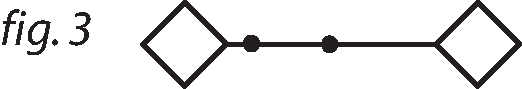
\includegraphics[%trim = -3mm -2mm 0mm 0mm, clip,
width=0.27\textwidth]
{images/LH037,05_208v-d3.pdf}, {}]
\indent Perinde ut si quod esset firmum, sed duobus in diversa trahentibus in duobus extremis alligatum, rumpetur \edtext{simul in}{\lemma{22f.\hspace{1.8mm}simul in}\killnumber\Bfootnote{\textit{(1)} diversis \textit{(2)} duobus \textit{L}}} 
\end{window}
\noindent duobus 
%\begin{wrapfigure}[3]{l}{0.27\textwidth}
%\vspace{-1mm}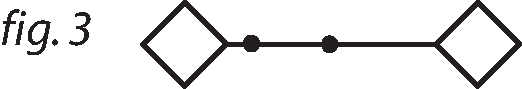
\includegraphics[trim = 0mm 0mm -5mm 0mm, clip,width=0.27\textwidth]{images/LH037,05_208v-d3.pdf}
%% \newline%
%% \rule[0pt]{15mm}{0mm}[\textit{Fig. 3}]
%\end{wrapfigure}
%Perinde ut si quod esset firmum, sed duobus in diversa trahentibus in duobus extremis alligatum, rumpetur \edtext{simul in duobus}{\lemma{simul in}\Bfootnote{\textit{(1)} diversis \textit{(2)} duobus \textit{L}}} 
\setline{23}illis extremis, (sed opus est ad rupturam\protect\index{Sachverzeichnis}{ruptura} vi duplicata, ejus qua opus foret si uno tantum loco esset alligatum). Perinde enim est ac si trahens ibi immediate alligatum esset, ubi infirmum est, in quo fit ruptura\protect\index{Sachverzeichnis}{ruptura}. Unde intelligitur si non punctum sit debile sed recta integra continua, in ejus medio fieri rupturam\protect\index{Sachverzeichnis}{ruptura}. Quod si duae sint lineae infirmae aequales inaequalesve, item aequaliter inaequaliterque a trahentibus remotae. Ruptura\protect\index{Sachverzeichnis}{ruptura} fieri debet in medio utriusque, opinor. Id enim fieret in qualibet si altera non adesset. Jam \setline{1}non est ratio cur altera alteri praeferatur.
\pend
\vspace*{1.5em}
\pstart
\noindent
\centering
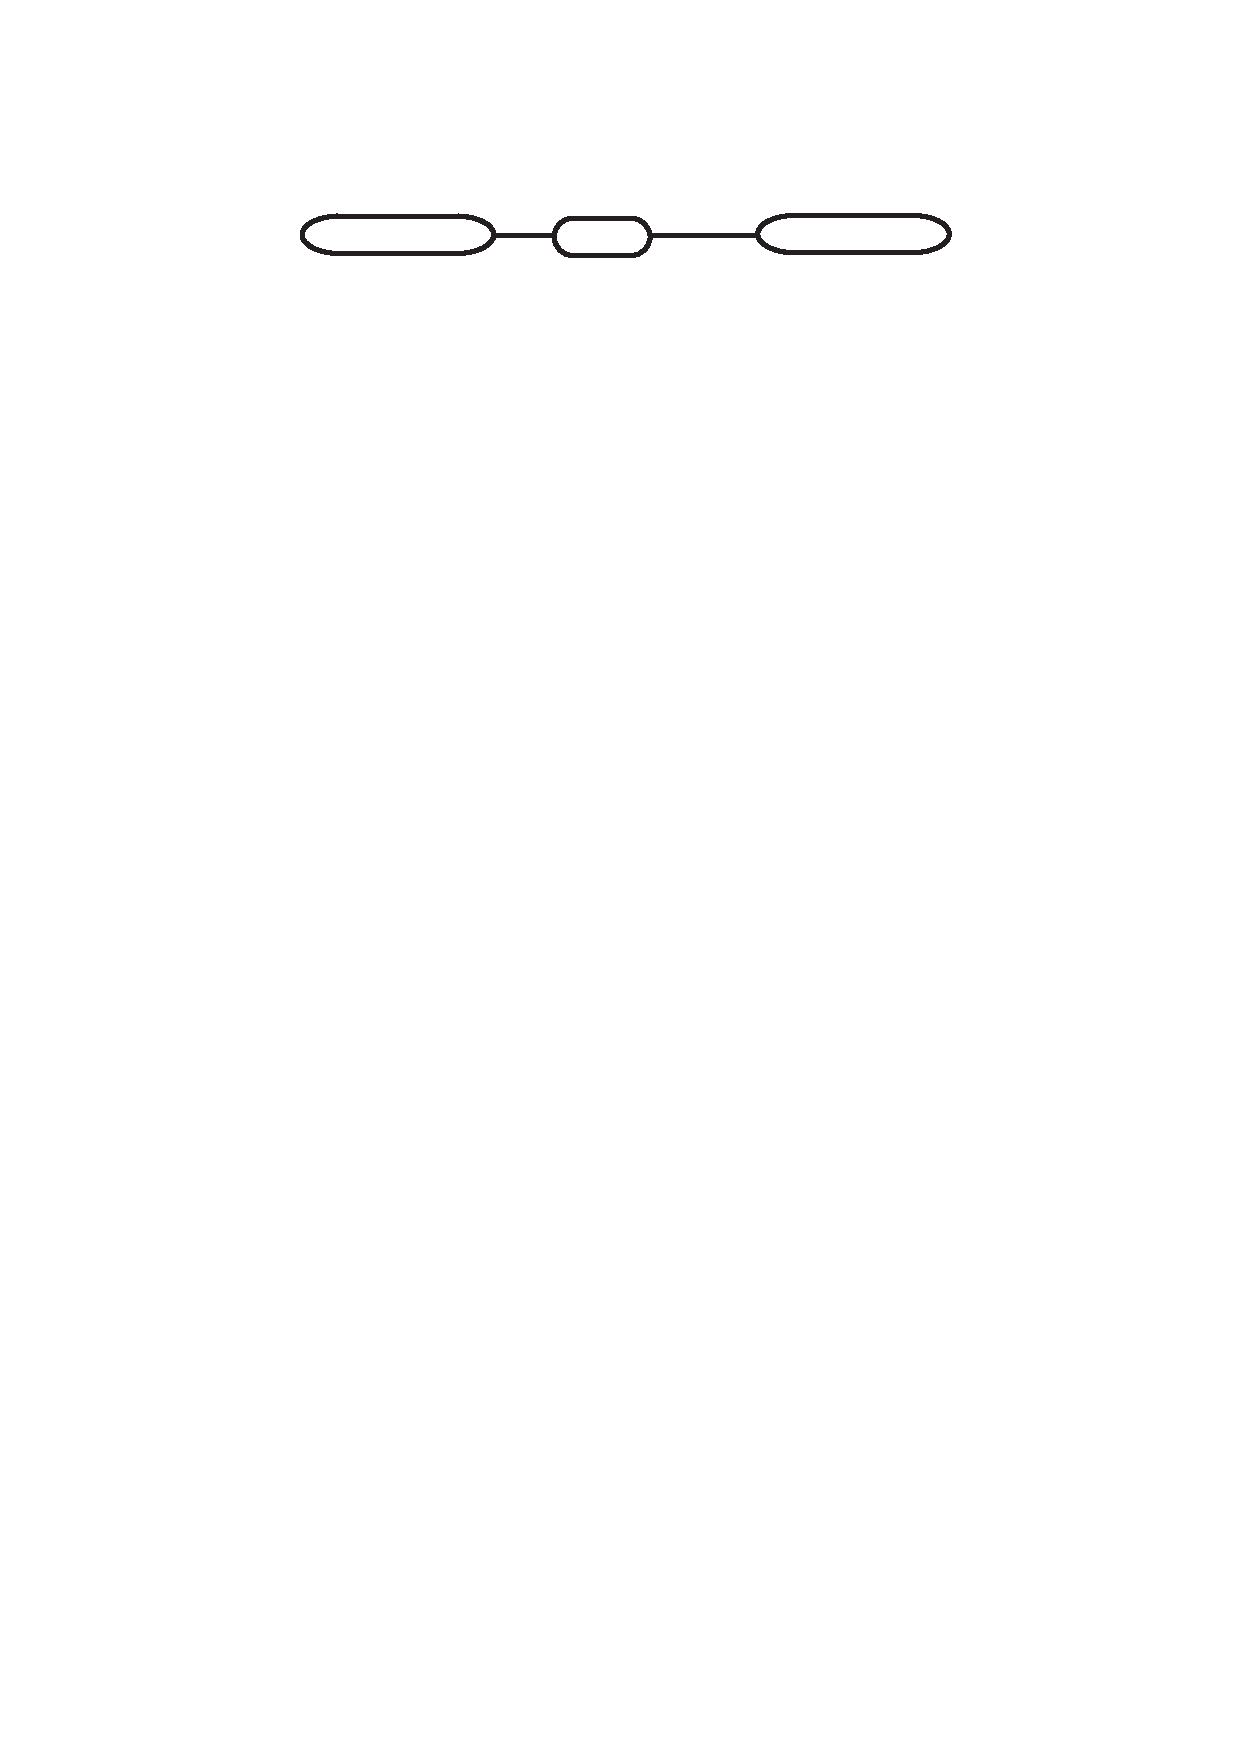
\includegraphics[trim = 0mm -3mm 0mm 0mm, clip, width=0.35\textwidth]{images/lh03705_208v-d4.pdf}\\
\centering
[\textit{Fig. 4}]
\pend
\vspace{1.5em}
\pstart%
Si nodus sit extra medium
\raisebox{-1,5ex}% PR: Rein provisorisch !!!
{\includegraphics[width=0.22\textwidth]{images/lh03705_208v-d5.pdf}} [\textit{Fig. 5}]
quaeritur ubi futura sit ruptura\protect\index{Sachverzeichnis}{ruptura} an in medio quasi non adesset nodus, an in duobus nodi juncturis.
An vero computabitur Nodus in medio eligendo, quasi ipse quoque pars debilis esset.
\pend
\vspace{1.5em}% PR: Rein provisorisch !!!
\pstart%
\centering%
\noindent%
\includegraphics[width=0.55\textwidth]{images/lh03705_208v-d6u7u8.pdf}\\
\centering
[\textit{Fig. 6}]
\pend
\vspace*{1.5em}% PR: Rein provisorisch !!!
\pstart%
\noindent%
\begin{wrapfigure}[16]{l}{0.35\textwidth}
\vspace{-5mm}\includegraphics[trim = 0mm -3mm -5mm 0mm, clip, width=0.35\textwidth]{images/lh03705_208v-d9u10.pdf}\\
\centering[\textit{Fig. 7}]
\end{wrapfigure}
%\pend
%\newpage% PR: Rein provisorisch !!!
% \vspace*{1.0em}% PR: Rein provisorisch !!!
%\pstart%
Vis\setline{7} \edtext{trahens conatur attrahere}{\lemma{}\Bfootnote{trahens \textbar\ non \textit{gestr.} \textbar\ conatur \textit{(1)} rumpere \textit{(2)} attrahere \textit{L}}} tabulam primam sed trahere non
\edtext{potest, sine}{\lemma{potest,}\Bfootnote{\textit{(1)} in \textit{(2)} sine \textit{L}}} resistentia, nisi trahat secundam et cum hoc nihil obsit, trahit secundam, et eodem modo conatur trahere tertiam, sed non potest nisi vincat ejus cohaesionem cum muro, quia murum sequi non potest. Semper ergo ruptura\protect\index{Sachverzeichnis}{ruptura} ista fiet in ultimo.
Non potest dici conatus esse disjunctivos sunt enim omnes absoluti.
\newline
%\pend
%\pstart%
\hspace*{7.5mm}Si distrahatur in duo latera vi\protect\index{Sachverzeichnis}{vis} aequali tunc determinatur (1) \edtext{rupturam\protect\index{Sachverzeichnis}{ruptura} esse necessariam}{\lemma{rupturam}\Bfootnote{\textit{(1)} non posse \textit{(2)} esse \textit{(a)} universalem \textit{(b)} necessariam \textit{L}}}, (2) si quid assumatur pro uno trans medium assumendum et pro altero trans medium ab ipso. Jam unum non potest ire, quia alterum ei occurrat. (3) nec assumi debet cis medium, non enim est ratio ejus, aut est ratio, ut \edtext{generaliter ut}{\lemma{generaliter}\Bfootnote{\textit{(1)} pro \textit{(2)} ut \textit{L}}} supra de vi trahente pro \edtext{eorum}{\lemma{}\Bfootnote{ eorum \textit{ erg. L}}} maxime remoto seu medio totius. Hinc demonstratur, si nodus vel firmum aliquid occupet medium, in duabus cum eo juncturis ruptum iri. Sed si nodus sit extra medium, ruptura\protect\index{Sachverzeichnis}{ruptura} nihilominus fiet in medio. Nam in firmum illud seu nodum non est \edtext{conatus, non}{\lemma{conatus, }\Bfootnote{\textit{(1)} cum \textit{(2)} non \textit{L}}} ab $a$ remoto, quia destruitur a propinquo \edtext{quod est trans medium}{\lemma{}\Bfootnote{quod est trans medium \textit{erg. L}}}, non a propinquo quia est ni agit in remotissimum quod potest seu medium, non in caetera. Si nodus incidat in medium, at tamen medium non sit in medio nodi\protect\index{Sachverzeichnis}{nodus} seu firmi nihilominus ruptura\protect\index{Sachverzeichnis}{ruptura} erit in duabus juncturis, quia haec remotissima \edtext{possibilia}{\lemma{}\Bfootnote{possibilia \textit{erg. L}}} cis medium.
[207~r\textsuperscript{o}]
\pend
\pstart%
Si totum sit firmum praeter unum punctum extra medium in eo fiet ruptura\protect\index{Sachverzeichnis}{ruptura}. Si duo sint puncta debilia utraque cis medium vel trans medium (pro diverso distrahentium respectu) vel etiam plura, ruptura\protect\index{Sachverzeichnis}{ruptura} semper fiet in eo quod medio proximum est.
\pend
\pstart
Si inaequales sint vires distrahentes, et aequalis sit firmitas aut debilitas fili.
Sed praedecidenda alia quaestio:
Si quid attrahat filum\protect\index{Sachverzeichnis}{filum} \edtext{ex}{\lemma{}\Bfootnote{ex \textit{erg. L}}} duabus partibus tenuiore et crassiore compositum, quaeritur qualis sit junctura tenuioris cum crassiore, an sit differentia utriusque. Est tenuior. 
\pend 
\pstart Deinde \edtext{si duo sint debilia}{\lemma{si}\Bfootnote{\textit{(1)} duae sint firmita \textit{(2)} duo sint debilia \textit{L}}} in filo attracto loca, alter tamen altero debilior, et firmior sit remotior a trahente, nihilominus tamen superabilis, an cedat debilior, ita sane cedit, nec firmior rumpitur, dum in debiliore exitus inveniri potest. Nec refert dicere, nullum esse conatum in propinquiora, cum scilicet nullum in illis lucrum. Ergo ex duabus consistentiis aequalibus semper conatus in remotiorem.
\pend
\pstart%
Si inaequales sunt vires\protect\index{Sachverzeichnis}{vis} distrahentes, rumpiturne in reciproca ad vires distantia. Ita arbitror. Medium ergo intelligendum proportionis seu Geometricum. Hoc difficile demonstratu.
\pend
\pstart%
Si duo trahant, ruptura\protect\index{Sachverzeichnis}{ruptura} fit viribus tantis quanta \edtext{est utriusque}{\lemma{}\Bfootnote{est \textbar\ est \textit{streicht Hrsg.} \textbar\ utriusque \textit{L}}} simul.
\pend
\vspace{1.5em}% PR: Rein provisorisch !!!
\pstart%
% \begin{wrapfigure}{l}{0.3\textwidth}
\centering%
\noindent%
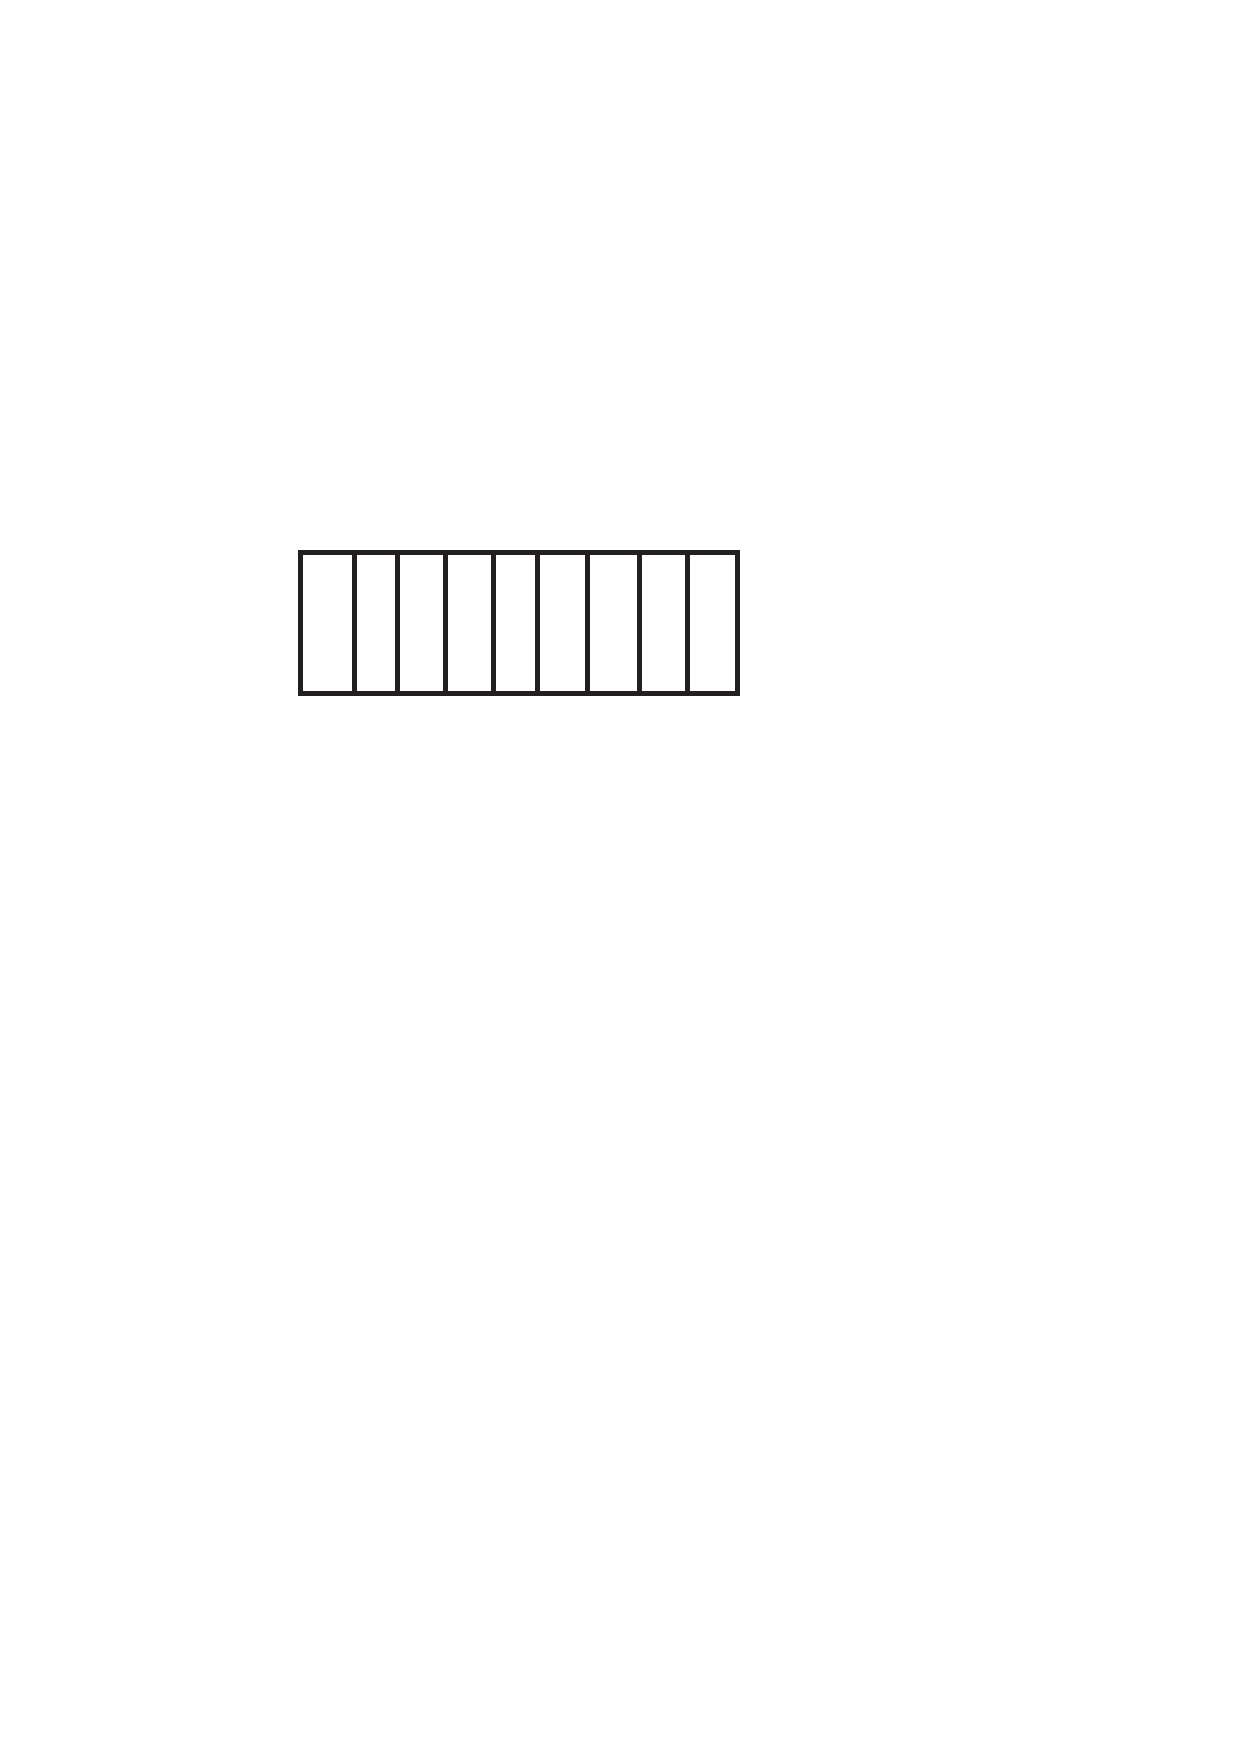
\includegraphics[width=0.3\textwidth]{images/lh03705_207r-d1.pdf}\\
\centering[\textit{Fig. 8}]
% \end{wrapfigure}
\pend
\vspace{1.5em}% PR: Rein provisorisch !!!
\pstart%
Si fit\setline{23} in medio a duabus inaequaliter trahentibus, fiet etiam in medio altero pene nihil trahente, seu quasi penitus quiescente, contra probata. Si fit in extremo, fiet etiam in extremo viribus pene penitus aequalibus. Contra priora. Fiet ergo pro ratione extremorum.
\pend
\newpage
\pstart
Non est hoc demonstrandi genus quale vellem, ostensivum, deducit enim tantum ad absurdum, sed \edtext{nondum intimiora}{\lemma{nondum}\Bfootnote{\textit{(1)} solidio \textit{(2)} intimiora \textit{L}}} reperio.
\pend
\pstart
Hinc si lignum\protect\index{Sachverzeichnis}{lignum} rumpitur centraliter quidem sine fulcro tamen rumpetur non in medio, \edtext{sed centro}{\lemma{sed}\Bfootnote{\textit{(1)} centrum \textit{(2)} centro \textit{L}}}, ac proinde sectio erit in reciproca ab extremis virium ratione\protect\index{Sachverzeichnis}{vis}.
Idem est et si rumpitur non sit linea recta, sed arcus circuli.
Sed an idem si sit arcus Ellipseos\protect\index{Sachverzeichnis}{ellipsis} et Hyperbolae\protect\index{Sachverzeichnis}{hyperbola} etc.
Puto, nisi scilicet aequaliter distent ambae a vertice istarum figurarum, si sic
\raisebox{-3.25ex}{\includegraphics[width=0.10\textwidth]{images/lh03705_207r-d2.pdf}} \![\textit{Fig. 9}]\,
an semper pro medio habendum $a$.
% \pend
% \pstart%
\edtext{Ergo an et in}{\lemma{Ergo}\Bfootnote{\textbar\ an \textit{erg.} \textbar\ et in \textit{L}}}
Hyperbola\protect\index{Sachverzeichnis}{hyperbola} vel
Ellipsi\protect\index{Sachverzeichnis}{ellipsis} vertex $a.\ b$%
\ \raisebox{-4.8ex}{\includegraphics[width=0.15\textwidth]{images/lh03705_207r-d5.pdf}}\ [\textit{Fig. 10}]%
\ an et \edlabel{trabibus1}$c.d$.%
\edtext{}{{\xxref{trabibus1}{trabibus2}}\lemma{et $c.d.$}\Bfootnote{\textit{(1)} $\displaystyle\frac{a}{a+b}$ \textit{(2)} $\displaystyle\frac{a+b}{a}$ \textit{L}}}
\pend
\vspace*{2.0em}% PR: Rein provisorisch !!!
\pstart\noindent%
$\displaystyle\frac{a+b}{a}$%
\edlabel{trabibus2}%
\rule[-4mm]{0pt}{10mm}%
$\quad\displaystyle\frac{c+d}{c}%
\quad%
\displaystyle\frac{c^2+d^2+[2]cd}{c^2}$%
\edtext{}{\lemma{2}\Bfootnote{\textit{erg. Hrsg.}}}%
\setline{1}%
\pend
%\newpage% PR: Rein provisorisch !!!
\vspace*{3.5em}% PR: Rein provisorisch !!!
\pstart
\begin{minipage}[t]{0.5\textwidth}
\noindent
\centering
\hspace{-16mm}
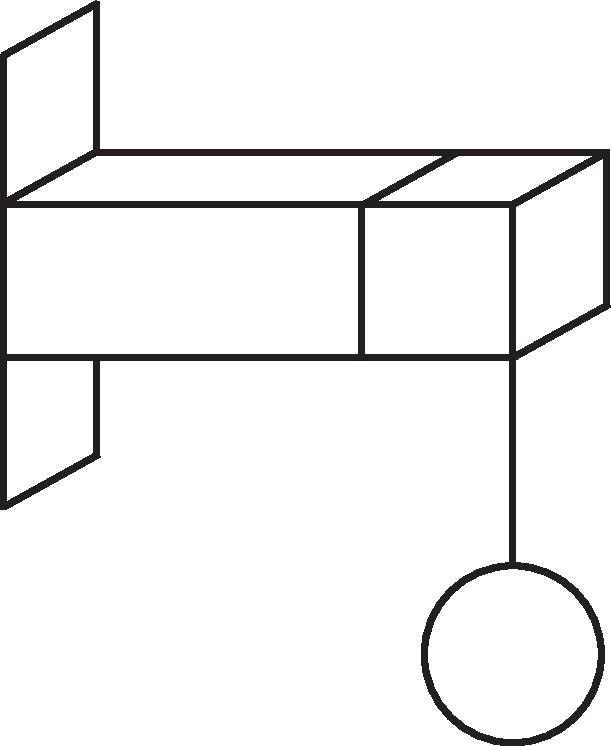
\includegraphics[width=0.5\textwidth]{images/LH037,05_207r-d3.pdf}
\\
 \vspace*{0.5em}
\hspace{-16mm}
[\textit{Fig. 11}]
\end{minipage}
\begin{minipage}[t]{0.5\textwidth}
\noindent
\centering
\hspace{-16mm}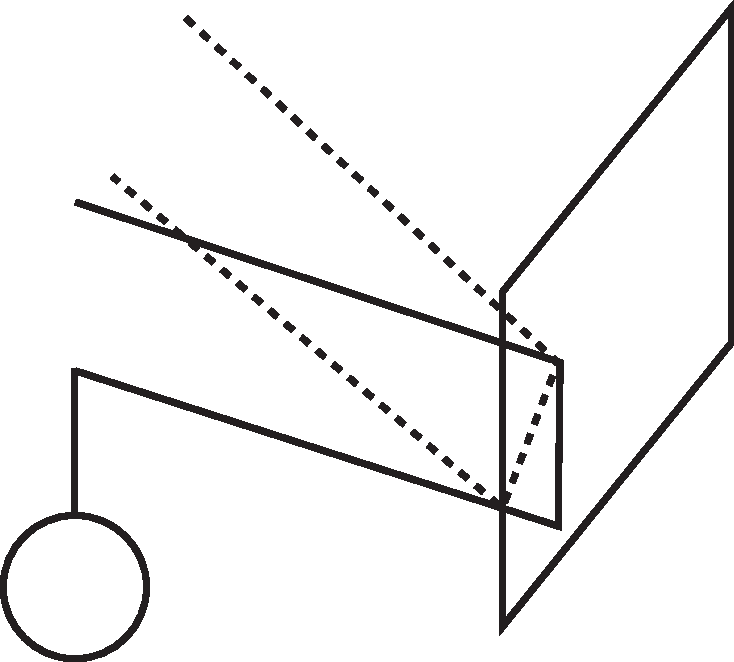
\includegraphics[width=0.60\textwidth]{images/LH037,05_207r-d4.pdf}
\\
 \vspace*{0.5em}
\hspace{-16mm}% PR: Rein provisorisch !!!
[\textit{Fig. 12}]
\end{minipage}
\pend
\newpage
%
%\vspace*{3.0em}% PR: Rein provisorisch !!!
%
\pstart
\begin{minipage}[t]{0.5\textwidth}
\noindent
\centering
\hspace{-16mm}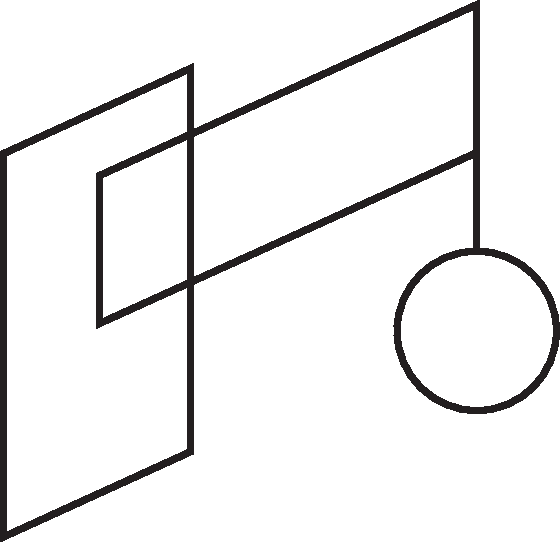
\includegraphics[width=0.45\textwidth]{images/LH037,05_207r-d6.pdf}
\\
 \vspace*{0.5em}
\hspace{-16mm}[\textit{Fig. 13}]
\end{minipage}
\begin{minipage}[t]{0.5\textwidth}
\noindent
\centering
\hspace{-16mm}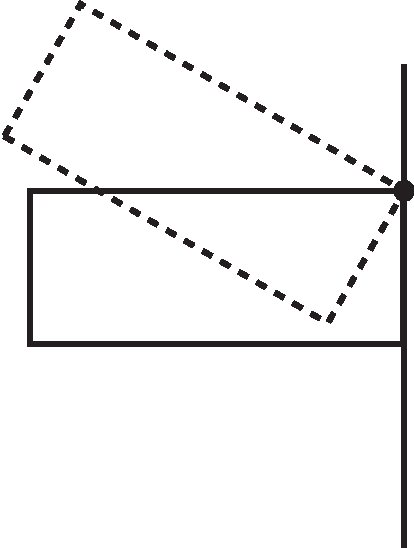
\includegraphics[width=0.37\textwidth]{images/LH037,05_207r-d7.pdf}
\\
 \vspace*{0.5em}
\hspace{-16mm}[\textit{Fig. 14}]
\end{minipage}
% \begin{center}
% 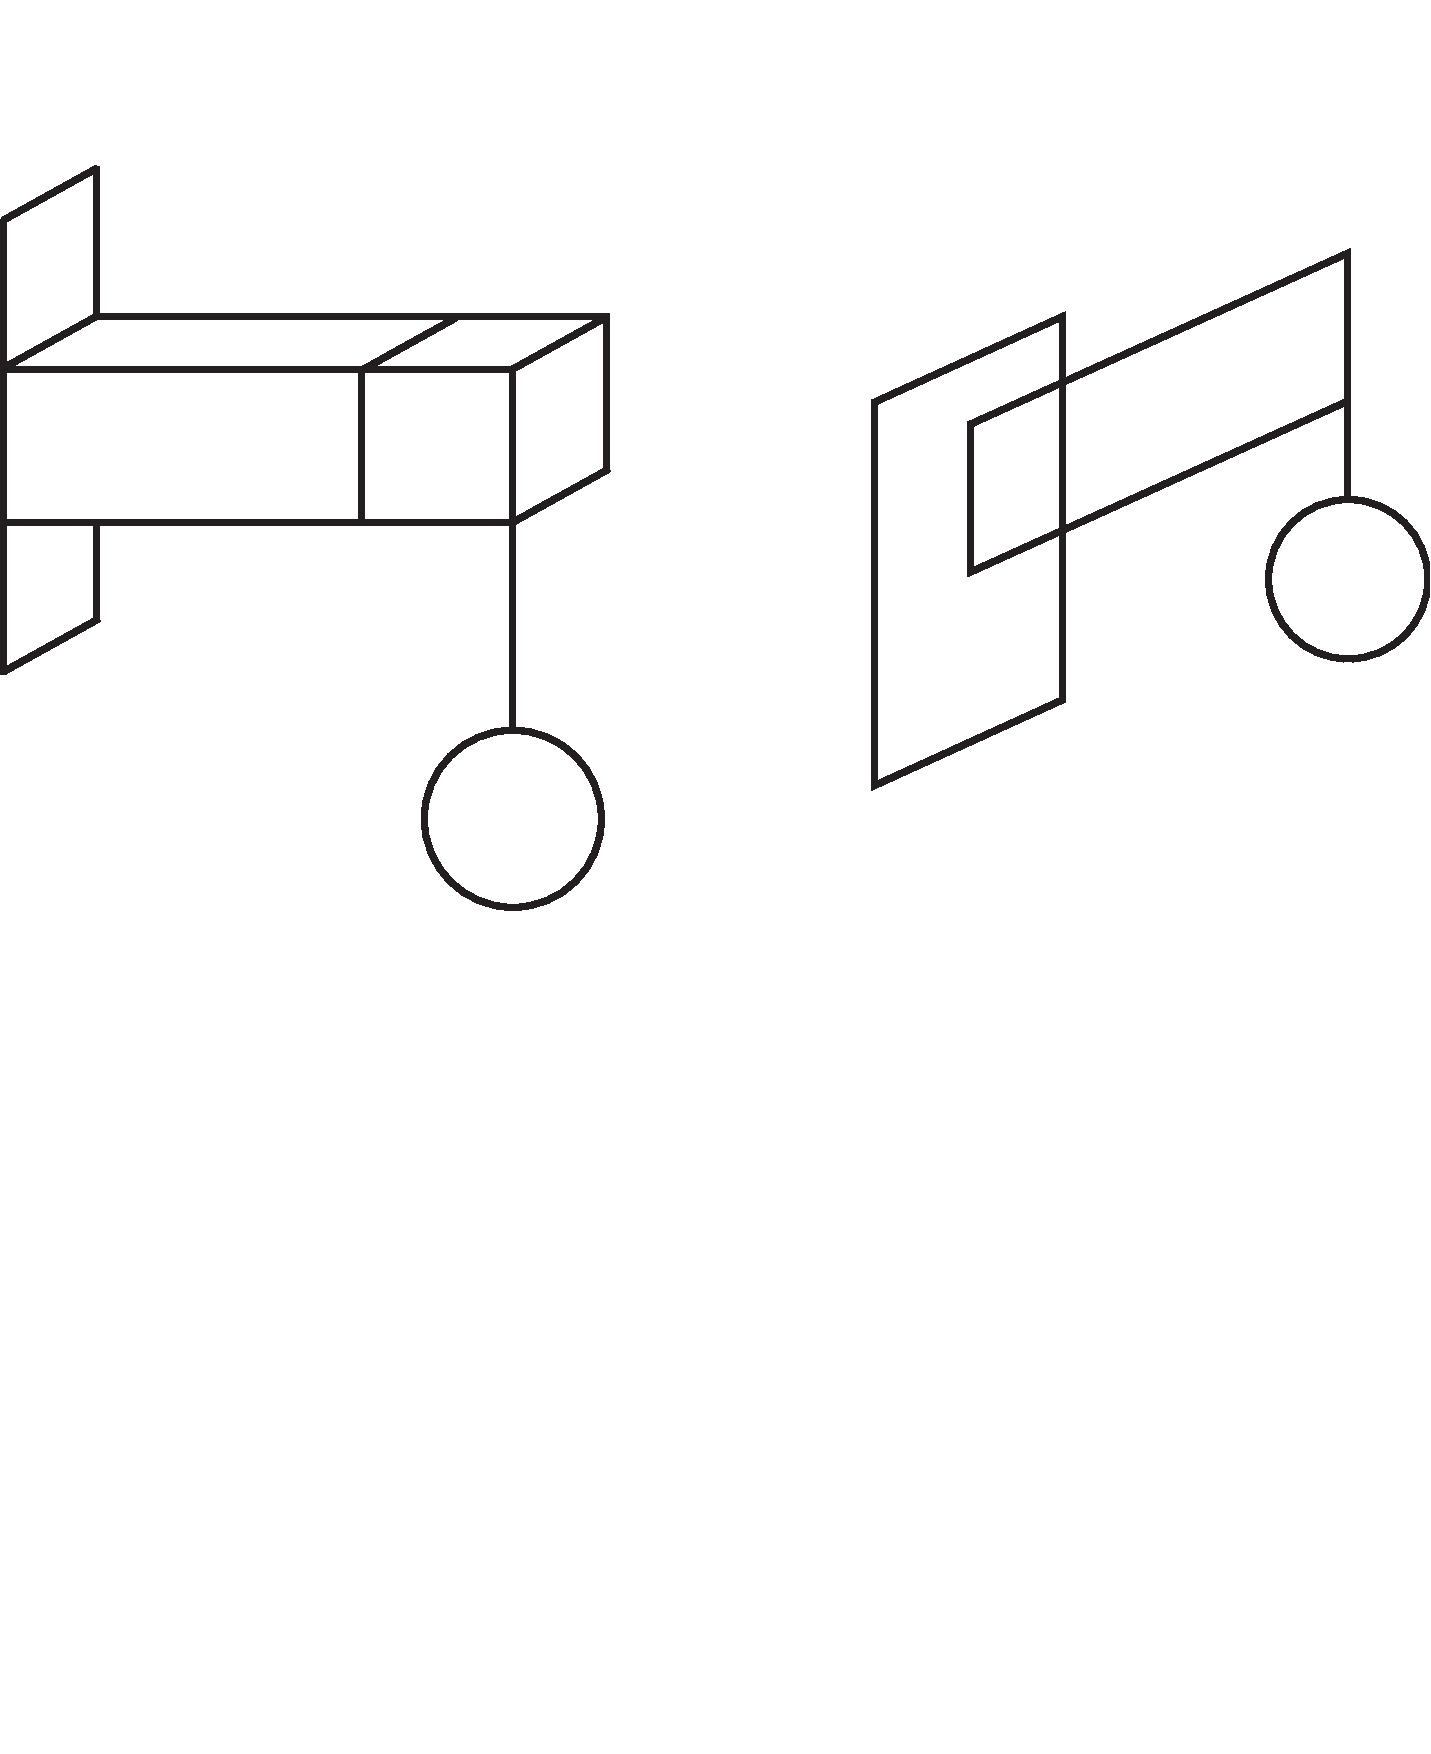
\includegraphics[width=0.6\textwidth]{images/lh03705_207r-d3u6.pdf}\\
% \rule[0pt]{10mm}{0mm}[\textit{Fig. 11}]\rule[0pt]{30mm}{0mm}[\textit{Fig. 12}]\\
% 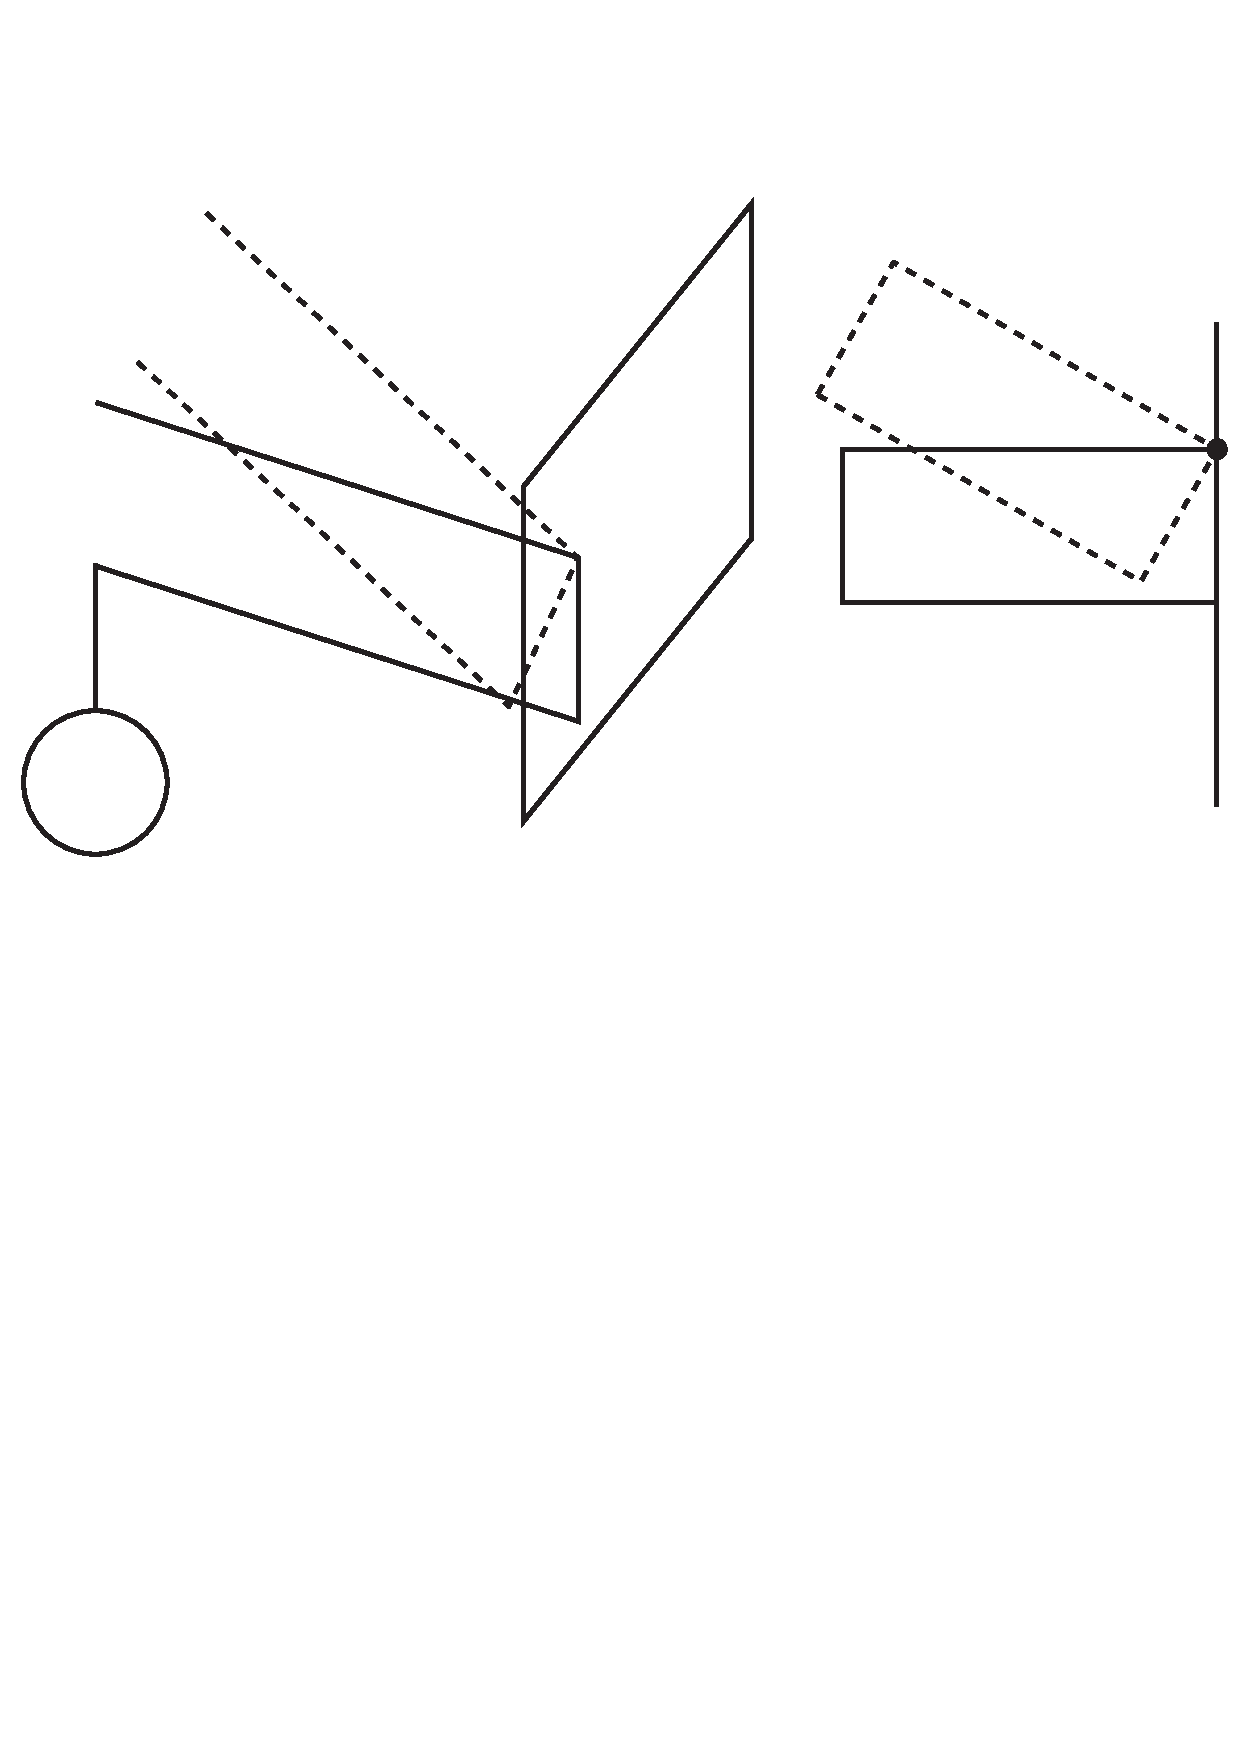
\includegraphics[width=0.6\textwidth]{images/lh03705_207r-d4u7.pdf}\\
% \rule[0pt]{10mm}{0mm}[\textit{Fig. 13}]\rule[0pt]{30mm}{0mm}[\textit{Fig. 14}]\\
% \end{center}
\pend
\vspace*{4.0em}% PR: Rein provisorisch !!!
% \newpage% PR: Rein provisorisch !!!
\pstart%
\noindent%
\textit{Ohne erkennbaren Zusammenhang mit dem Text:}\setline{1}
\pend
\vspace*{1.5em}%
\pstart%
\edtext{}{\lemma{}\Bfootnote{$2$ \textit{erg. Hrsg.}}}
$\begin{array}{rr} 3925 \\ 342 \\ \rule[2mm]{8mm}{0.4pt} \end{array}$ \hspace{2em}
$\begin{array}{cccccccc}
&&&\cancel{1}&[2]&&&\\
&&\cancel{0}&\cancel{8}&\cancel{9}&8&&\\
&\cancel{3}&\cancel{1}&\cancel{6}&\cancel{8}&\cancel{9}&2&\\
\cancel{1}&\cancel{3}&\cancel{4}&\cancel{2}&\cancel{6}&\cancel{3}&\cancel{2}& f.\ 3925\\
&\cancel{3}&\cancel{4}&\cancel{2}&\cancel{2}&\cancel{2}&\cancel{2}&\\
&&\cancel{3}&\cancel{4}&\cancel{4}&\cancel{4}&&\\
&&&\cancel{3}&\cancel{3}&&&\\
\end{array}$ %\advanceline{-2}
\pend
\count\Afootins=1500
\count\Bfootins=1500
\count\Cfootins=1500